\section{System Architecture}\label{sec:architecture}

PolyEdge is a full-stack autonomous trading system comprising a React 18 frontend, a Python FastAPI backend, and a multi-source data ingestion layer. The architecture follows a layered design in which data flows through ingestion $\to$ strategy generation $\to$ risk validation $\to$ debate validation $\to$ execution $\to$ settlement, with observability and autonomy loops wrapping the entire pipeline.

\subsection{Component Overview}

\textbf{Frontend.} The dashboard is built in React 18 with TypeScript, TanStack Query for server-state synchronization, Tailwind CSS for styling, and Vite for bundling. It provides real-time monitoring via Server-Sent Events (SSE) on \texttt{/api/events/stream}, WebSocket price ticks on \texttt{/ws/markets}, and whale alerts on \texttt{/ws/whales}. Key views include the dashboard overview (bankroll, equity, P\&L), admin controls (mode switching, experiment management), signals table, trades table, and a 3D globe visualization of market exposure.

\textbf{Backend.} The FastAPI application exposes REST endpoints for trading, market data, experiment management, and system health. The core engine coordinates nine strategies through an orchestrator that wires the Polymarket CLOB client, APScheduler, Telegram bot, and event bus. Strategies are auto-registered via a \texttt{@register\_strategy} decorator and stored in \texttt{StrategyConfig} rows in SQLite (or PostgreSQL in production). Each strategy returns a list of \texttt{TradingSignal} objects with confidence scores, edge estimates, and metadata.

\textbf{Data Sources.} Market data arrives from Polymarket (via the CLOB SDK and WebSocket), Kalshi (REST API), Coinbase/Kraken/Binance (BTC klines), Open-Meteo (GFS ensemble forecasts), and the National Weather Service (NWS API). A multi-source aggregator with fallback chains ensures continuity when individual feeds fail.

\subsection{Signal Flow}

The end-to-end signal flow is as follows (see Figure~\ref{fig:architecture}):

\begin{enumerate}
    \item \textbf{Market Data Ingestion.} The orchestrator initializes data feeds on startup. APScheduler runs interval jobs (BTC scan, weather scan, settlement check, arbitrage scan) that fetch live market data and store snapshots in the database.
    
    \item \textbf{Strategy Generation.} One of nine strategies processes the raw data and generates \texttt{TradingSignal} objects. Strategies include BTC momentum (RSI + VWAP on 1m/5m/15m candles), weather EMOS (31-member GFS ensemble temperature forecasting), copy trader (mirroring whale positions), Kalshi arbitrage (cross-platform price gaps), and a real-time scanner (price velocity detection).
    
    \item \textbf{Risk Validation.} Every signal passes through the \texttt{RiskManager}, which validates confidence, size, exposure, drawdown, and unsettled-position constraints. The manager returns a \texttt{RiskDecision} with an allowed flag, a human-readable reason (if rejected), and an adjusted position size. Risk profiles (safe, normal, aggressive, extreme) from ADR-005 overlay additional constraints that AI-generated strategies cannot bypass \citep{nygard2018release}.
    
    \item \textbf{Debate Validation.} High-confidence signals enter the MiroFish dual-debate system (detailed in Section~\ref{sec:debate}). Bull and Bear agents argue the merits of the trade; a Judge agent produces a verdict. Signals below the confidence threshold are rejected or queued for manual review.
    
    \item \textbf{Execution.} Approved signals flow to \texttt{strategy\_executor.execute\_decision()}, which either records a paper trade in the database or places a live CLOB order. The executor updates \texttt{BotState} (bankroll, equity, trade count) and publishes a \texttt{trade\_executed} event to the event bus.
    
    \item \textbf{Settlement.} When markets resolve, the settlement engine fetches final outcomes from the Gamma API, computes P\&L, handles partial settlements and tax-lot tracking, and updates trade rows. Unsettled positions are monitored continuously.
\end{enumerate}

\subsection{Infrastructure and Deployment}

The system runs on Docker Compose locally and deploys to Railway (backend) and Vercel (frontend) in production. Redis-backed job queues (with SQLite fallback) handle background strategy execution. Prometheus metrics endpoints provide request/response latency histograms. A PM2 process manager orchestrates multiple worker processes. All external API base URLs are configurable via environment variables, and feature flags (e.g., \texttt{WEATHER\_ENABLED}, \texttt{JOB\_WORKER\_ENABLED}) gate subsystems without code changes.

\subsection{Integration Points for the Three Contributions}

The three technical contributions described in this paper map directly onto architectural layers:

\begin{itemize}
    \item \textbf{Bounded AGI Autonomy} operates at the orchestration and scheduling layers. The \texttt{AutonomousPromoter} daemon, \texttt{StrategyHealthMonitor}, and \texttt{AGI\_\*} feature flags govern when strategies may run, how they are promoted, and when they are killed.
    \item \textbf{Evolutionary Strategy Composition} operates at the strategy layer. The \texttt{StrategyGenome} domain model and evolution operators (mutation, crossover, fitness) generate new strategy configurations that feed back into the orchestrator's strategy registry.
    \item \textbf{Dual-Debate Decision Validation} operates at the signal-validation layer. The MiroFish client intercepts \texttt{TradingSignal} objects after risk validation and before execution, adding a second opinion with structured reasoning.
\end{itemize}

These layers are decoupled: the debate system can be disabled without affecting strategy generation, and the autonomy framework can retire strategies without knowing their internal genome structure. This modularity ensures that each contribution can be evaluated, improved, or replaced independently.

\begin{figure}[H]
    \centering
    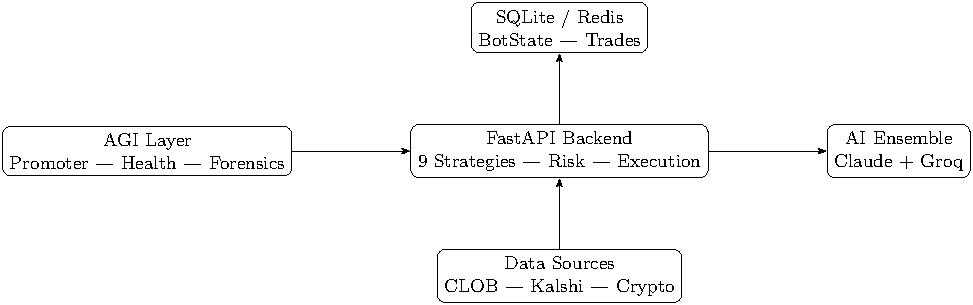
\includegraphics[width=0.95\textwidth]{figures/architecture.pdf}
    \caption{PolyEdge system architecture. The frontend (React 18) communicates via REST/WebSocket with a FastAPI backend. The core engine manages 9 strategies, an AGI intelligence layer (autonomous promoter, health monitor, forensics, bankroll allocator), and interfaces with Polymarket CLOB, Kalshi API, and crypto/weather data sources.}
    \label{fig:architecture}
\end{figure}
